\section{Day 9: Infinite Products, Metrics (Oct. 1, 2024)}
Outfit of the day! smth smth butterflies !!! very demure, very mindful
\begin{figure}[h]
    \centering
    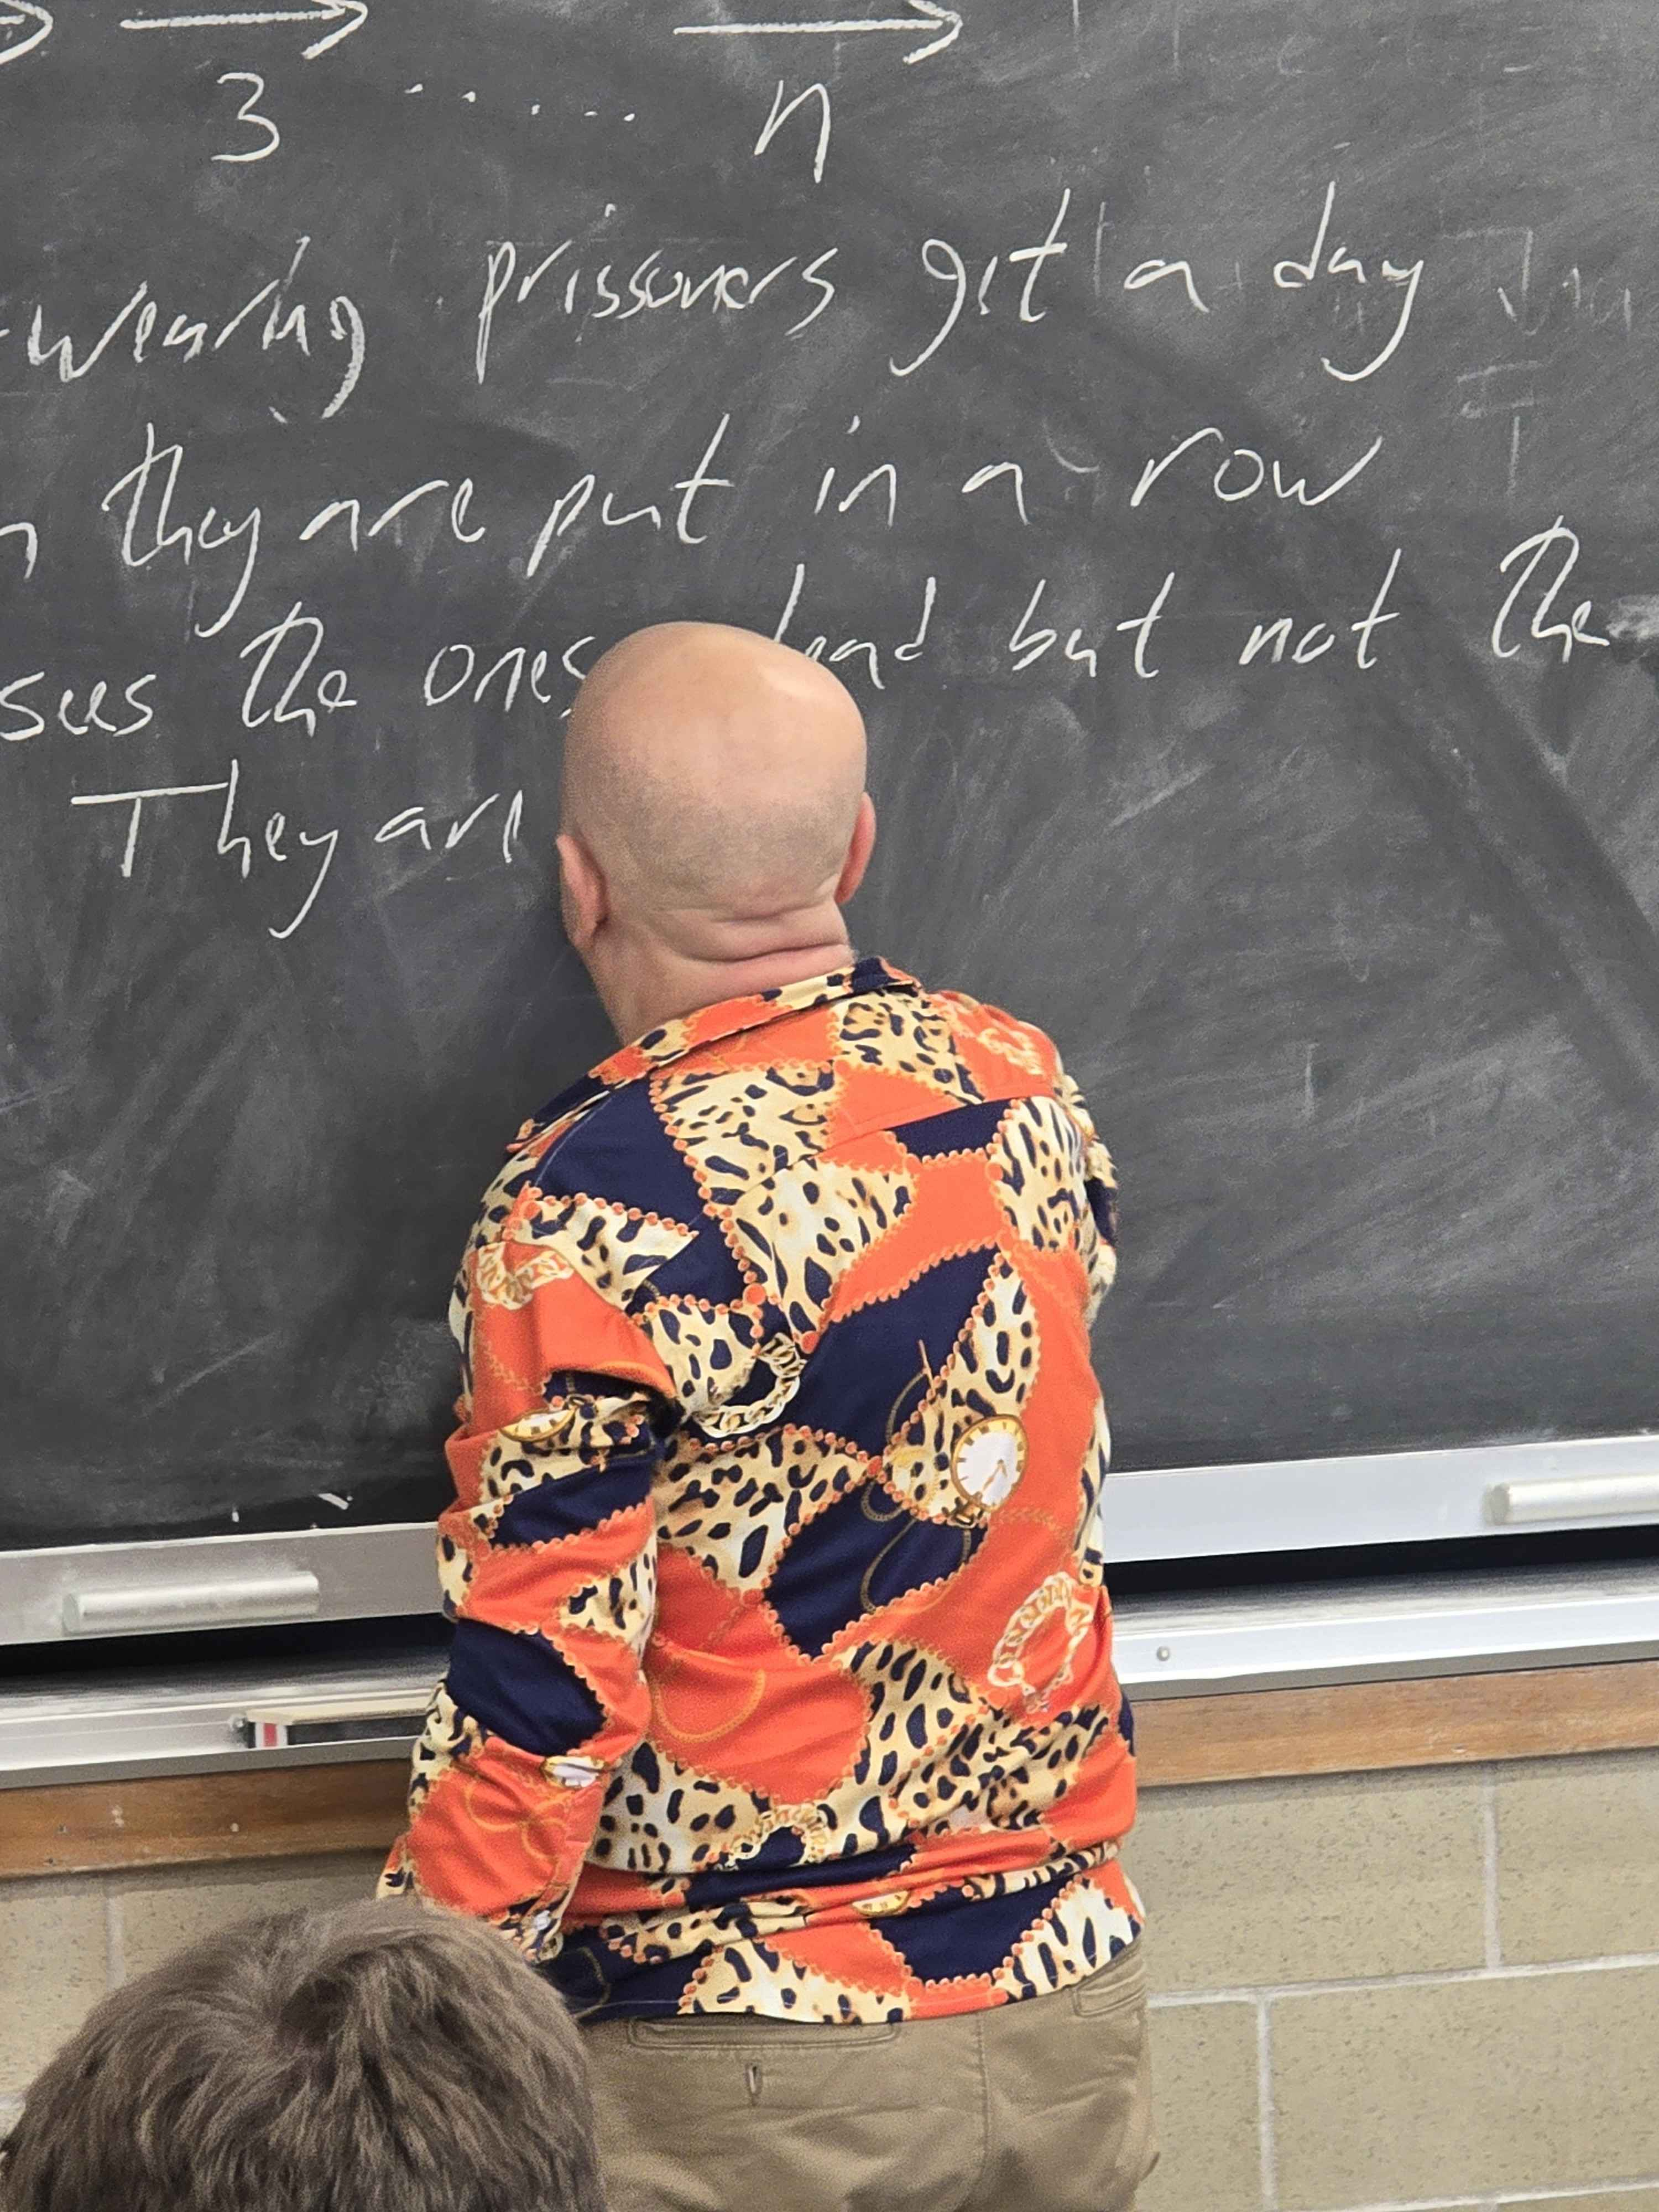
\includegraphics[scale=0.1]{MAT327 Notes/Dror Shirts/dror day 9 shirt.jpg}
\end{figure}

\noindent Recap of last lecture; topologies on $\prod_\alpha X_\alpha$ generalize the following;
\begin{enumerate}[label=(\alph*)]
    \item The basis $\SB_\mathrm{box} = \{\prod U_\alpha \mid U_\alpha \subset X_\alpha \text{ open}\} \rightsquigarrow \ST_\mathrm{box}$;
    \item The requirements $\SB_\mathrm{cyl} = \{\prod U_\alpha \mid U_\alpha \subset X_\alpha \text{ open}, \text{ almost always } U_\alpha = X_\alpha\} \rightsquigarrow \ST_\mathrm{cyl}$.
\end{enumerate}
Observe that the function sending a constant $t \in \RR$ to the constant sequence $(t, t, \dots) \in \RR^\NN$ is continuous in the cylinder topology, but not in the box topology (read: \href{https://en.wikipedia.org/wiki/Box_topology#Example_%E2%80%94_failure_of_continuity}{here}). This means $\ST_\mathrm{cyl} \supsetneq \ST_\mathrm{box}$ (in general, they are not the same); yet in both, both subspace and the Hausdorff property behaves (i.e., products preserve Hausdorff-ness).

\newpage
\begin{simpleclaim}[Theorem 19.5, Munkres]
    Let $\{X_\alpha\}$ be an indexed family of spaces, and let $A_\alpha \subset X_\alpha$ for each $\alpha$. Then we have that $\overline{\prod A_\alpha} = \prod \overline{A_\alpha}$ if $\prod X_\alpha$ is given the box or cylinder topologies.
\end{simpleclaim}
\noindent We prove this by double inclusion:
\begin{itemize}
    \item[$(\Leftarrow)$] Let $x = (x_\alpha) \in \overline{\prod_\alpha A_\alpha}$. Recall that $x$ is in the closure of $\prod A_\alpha$ if and only if every basic neighborhood of $x$ intersects $\prod_\alpha A_\alpha$. This condition is equivalent to saying that for all open neighborhood $U_\alpha \subset X_\alpha$, $x \in \prod U_\alpha \implies \prod U_\alpha \cap \prod U_\alpha \neq \emptyset$, which is also equivalent to saying that for all $\alpha$ where $x_\alpha \in U_\alpha$, we have $U_\alpha \cap A_\alpha \neq \emptyset$. Thus, every neighborhood $U_\alpha$ about $x$ intersect $A_\alpha$. This means for all $\alpha, x_\alpha \in \overline{A_\alpha}$, and we conclude that $x \in \overline{\prod_\alpha A_\alpha}$.
    \item[$(\Rightarrow)$] \textit{(Not covered in class)} Let $x = (x_\alpha)$ lie in the closure of $\prod A_\alpha$. Then for any index $\beta$, we have $x_\beta \in \overline{A_\beta}$. Let $V_\beta$ be an arbitrary open set of $X_\beta$ containing $x_\beta$. Since $\pi_\beta^{-1}(V_\beta)$ is open in $\prod X_\alpha$ in either topology, it contains $y = (y_\alpha) \in \prod A_\alpha$. Then $y_\beta$ belongs to $V_\beta \cap A_\beta$, which means $x_\beta \in \overline{A_\beta}$. \qed
\end{itemize}

\noindent We now move onto metric spaces. We say a metric on a set $X$ is a function $d : X \times X \to (\RR \geq 0)$ such that:
\begin{enumerate}[label=(\alph*)]
    \item $d(x, y) \geq 0$, with $d(x, y) = 0 \iff x = y$ (non-negativity);
    \item $d(x, y) = d(y, x)$ (symmetry);
    \item $d(x, z) \leq d(x, y) + d(y, z)$ (triangle inequality).
\end{enumerate}
\noindent We also define that $B_r(x_0) = \{x \mid d(x_0, x) < r\}$. Note that balls in non-euclidean metrics may look different from a sphere; we now give some examples of metrics:
\begin{enumerate}[label=(\alph*)]
    \item The Euclidean metric ($L^2$) on $\RR^n$, $d(x, y) = \sqrt{\sum_{i=1}^n (x_i - y_i)^2}$.
    \item The Manhattan distance ($L^1$) on $\RR^n$, $d(x, y) = \sum_{i=1}^n \abs{x_i - y_i}$. Note that here, a ball looks more like a fucked-up rhombus.
    \item For any set $X$, let us define $d(x, y) = 1$ for $x \neq y$, and $d(x, y) = 0$ if $x = y$.
    \item For bounded sequences $(a_i) \in \RR^\NN$, we may define $d(a, b) = \sup \abs{a_i - b_i}$ (aka $L^\infty$).
\end{enumerate}
A set with a metric on it is called a \textit{metric space}; on metric spaces, we set $\SB_\mathrm{d} = \{B_r(x_0)\}$, i.e. the set of all open balls, and we claim that this is indeed a basis \textit{(Left as exercise, but it's obvious)}. In particular, every metric space has a topology; namely, it is a topological space; we claim that the metrics introduced above induce the same topology, i.e. the discrete topology on $\RR^n$, except (d).
\medskip\newline
\noindent All metric spaces are Hausdorff by considering the triangle inequality.